\chapter{Getting Started} \label{sec:basics}

\section{Requirements}

\subsection{Downloading Mesquite}
The Mesquite distribution (in source form) may be obtained at the following URL:
\begin{verbatim}
http://www.cs.sandia.gov/~web9200/
\end{verbatim}

\subsection{Supported Platforms and Build Requirements}
The Mesquite source code will compile in any environment comforming to the ISO/IEC 9899-1999 (C99), ISO/IEC 14882-1998 (C++98) and ISO/IEC 9945:2003 (POSIX) standards.
It may also compile under many other environments.

Mesquite requires a reasonably standards-conforming C++ compiler and corresponding libraries.  No additional libraries are required to build the core Mesquite library.
Several optional features have additional requirements.  These are listed in the next section.

Mesquite includes a build system that should work on most Unix-based or Unix-like
operating systems.  The Unix build system provided for Mesquite requires the GNU implementation of the \texttt{make} utility.  It may be obtained at this URL:
\begin{verbatim}
http://ftp.gnu.org/pub/gnu/make/
\end{verbatim}

Support for building Mesquite with Microsoft Visual Studio (version 6.0 or later) is provided via Visual Studio project and workspace files.

Mesquite is regularly compiled and tested on GNU/Linux with g++ 3.2 or later and Sun with the Sun Forte C++ compiler.  

\subsection{Optional Libraries and Utilities}
\label{sec:depends}
\begin{itemize}
\item Unit tests:  Mesquite provides a series of unit tests that may be used
to verify the correct behavior of a build of the Mesquite library.  These tests
are implemented using CppUnit framework.  The CppUnit framework must be installed
to compile and run these test.  It is available at this URL:
\begin{verbatim}
http://cppunit.sourceforge.net
\end{verbatim}
\item TSTT SIDL interface:  A working Babel/SIDL installation (version 0.9.8 or 
newer) is requred for building the interface objects that allow Mesquite to
directly access Mesh stored in an implementation providing the TSTT mesh interface.  Babel/SIDL can be obtained at this URL:
\begin{verbatim}
http://www.llnl.gov/CASC/components/software.html
\end{verbatim}
\item ExodusII support:  To enable support for reading or writing ExodusII files in Mesquite, the header files for the ExodusII library must be available.  To link an application with a Mesquite library supporting ExodusII, the ExodusII library and possibly the NetCDF library must be available.  To obtain the ExodusII library, contact:
\begin{verbatim}
Marilyn K. Smith
Research Programs Department
Department 9103, MS 0833
Sandia National Laboratories
P.O.Box 5800
Albuquerque, NM 87185-0833
Phone: (505) 844-3082
FAX:   (505) 844-8251
Email: mksmith@sandia.gov
\end{verbatim}
The NetCDF library can be obained at the following URL:
\begin{verbatim}
http://my.unidata.ucar.edu/content/software/netcdf/index.html
\end{verbatim}
\end{itemize}


\section{Building Mesquite}
\label{sec:compiling}
After downloading and unpacking the Mesquite source, the next step is to 
configure and build the Mesquite library (libmesquite.a on Unix-like systems or 
mesquite.lib on Windows.)
\subsection{Compiling on Unix-like systems}
This section presents the steps required to compile Mesquite with the default
options.  Mesquite requires the GNU implementation of the \texttt{make} utility.
On some systems the command to invoke GNU make may be \texttt{gmake}.  Substitute
\texttt{gmake} or whatever the command is on your system for GNU make in place of
the \texttt{make} command in the instructions below.
\begin{enumerate}
\item Make the working directory of your command shell the top-level Mesquite
directory (typically \texttt{mesquite/}).
\item Run the configure script with the command: \texttt{./configure}
\item Compile Mesquite with the command: \texttt{make} 
\item Verify that Mesquite compiled correctly with the command: \texttt{make test}
\end{enumerate}
If the configure step failed, please consult the following section describing 
some of the optional arguments to the \texttt{./configure} script. 
\subsection{Options for Unix-like systems}
This section describes the options available for customizing the build
system and the resulting Mesquite library.  An brief description of these
and other options is available with the command: \texttt{./configure --help}.

\label{mes_vars_and_defs}
The following values may be specified as environmental variables, as arguments
to the configure script using the NAME=VALUE syntax, or as arguments to \texttt{make}
using the NAME=VALUE syntax.  The value of these variables (if set) during the
configure step will become the default for the compile step.  The value of any
of these variables will override the the default if specified during the compile
step.
\begin{description}
\item[CXX]       The C++ compiler command
\item[CXXFLAGS]  Arguments to the C++ compiler, such as those specifying 
debug symbols or the optimization level.
\item[CC]        The C compiler command
\item[CFLAGS]    Command line arguments to be used for the C compiler.
\end{description}

Most options to the configure script are either of the form \texttt{--with-FEATURE[=ARG]} or
\texttt{--enable-FEATURE[=ARG]}.  Some options may accept an additional argument following 
an '=' character.  For each --with-FEATURE option, there is also a corresponding
--without-FEATURE option.  Similarly, there is a --disable-FEATURE option 
corresponding to each --enable-FEATURE option.  The negative forms fo the options 
(--without-FEATURE and --disable-FEATURE) do not accept an additional argument.  
Only the positive form of each option is stated in the description below.  

\label{config_options}
The following general build and debug options may be specified during the configure step:
\begin{description}
\item[--with-archiver=ARG]  This option may be used to specify the
system-specific command to generate a static library (archive) from a group
of compiled object (.o) files.  Use this option if the \texttt{./configure} script fails to correctly detect the archiver command.
\item[--enable-debug]  Select a subset of the following options that
make the most sense for developers of Mesquite.
\item[--enable-release]  This is the default behavior unless 
--enable-debug is specified.  It selects a subset of the following options that
typically work best for using Mesquite in a production application.
\item[--enable-compile-optimized] Compile with the available 
optimizations that improve performance without any significant drawbacks 
(the -O2 compiler flag.)
\item[--enable-debug-symbols] Include debugging information in
the compiled Mesquite objects (the -g compiler flag).
\item[--enable-debug-assertions]  Include internal consistancy 
checks that abort when an error is detected.
\item[--enable-debug-output=n,m,...]  Enable the output of
debug and status messages to file descriptor 1 (stdout).  An 
list of integer debug flags for which to enable output may be specified 
as a comma-separated list of values.  The default is to enable debug
flags 1 and 2 if this option is specified without any explict debug
flag values.
\item[--enable-function-timers]  Enable time-profiling of
some portions of Mesquite.
\item[--enable-trap-fpe]  Enable generation of a floating-point
exception signal for arithmatic errors (e.g. division by zero.)  This is
an option intended for Mesquite developers.  Enabling this will typically cause
the application using Mesquite to abort when such an error is encountered.
\end{description}

The following options specify optional Mesquite components and the location 
of the corresponding dependencies.
\begin{description}
\item[--with-doxygen=PROG] Specify the location of the Doxygen
command for generating developer documentation.
\item[--with-cppunit=DIR]  The CppUnit library is required to compile
and run the tests to verify that a particular build of the Mesquite library
is working correctly.  If the CppUnit library is not installed in a default location
where the ./configure script can find it, this option may be used to specify
the location.
\item[--with-exodus=DIR]  Enable support for reading and writing
ExodusII files, and optionally specify the location where the ExodusII library
and headers required for this option are installed.
\item[--with-netcdf=DIR]  Specify the location of the NetCDF library
required by the ExodusII library.  The default is to look in the ExodusII
directory.
\item[--enable-tstt]  Enable optional support for accessing mesh
and geometry data through the TSTT SIDL interfaces.  This option requires
the Babel utility for processing SIDL files.
\item[--with-babel=DIR]  Specify the location where the Babel/SIDL
package is installed.
\end{description}

\subsection{Compiling on Microsoft Windows}
The Mesquite source package includes project and workspace files for Microsoft Visual C++ 6.0 or later.  To build Mesquite in Visual C++:
\begin{itemize}
\item Open the file: \texttt{mesquite/mswindows/mesquite.dsw}
\item Select between a debug or release build in the project settings.  
\item Set the active project to \texttt{mesquite}
\item Select \texttt{Build mesquite.lib} from the \texttt{Build} menu.
\end{itemize}

\section{Short Tutorial}

In this section, we write a driver code which calls the Mesquite
library to improve the quality of a test mesh. This tutorial section
is aimed at giving the user a feel for Mesquite: \emph{this section is not
where to look for detailed information}. In particular, information
pertaining to loading a particular mesh format (see section X), 
interacting through a particular mesh interface (section Y), 
and details of the API classes (sections 4.X-4.Y) are not
given in this section.

First, we write a small program using Mesquite's simplified API, or
wrappers, to show the fastest way deploy Mesquite functionality to
improve a mesh.  The wrapper concept, as well as details about the
different wrappers available, are described in section
\ref{sec:wrappers}.  Following this first example, we set up customized mesh
improvement tool using Mesquite's low-level API, the details of which
are described in section \ref{sec:detailedAPI}.

\subsection{Tutorial File Template}
\label{sec:tutfile}

To create and link a driver code, the Mesquite library must be
compiled per the instructions of section \ref{sec:compiling}. 
This tutorial begins with the file \newline
\texttt{testSuite/tutorial/tutorial.cpp}, 
which contains the following template:
\begin{verbatim}
1.   #include "Mesquite_all_headers.hpp"
     #include <ostream>
2.   using namespace Mesquite;
     int main(int argc, char* argv[])
     {
3.      MsqError err;
  
        char mesh_file_name[256];
  
        // command line arguments
        if (argc==1 || argc>2) {
          std::cerr << "meshfile name needed as argument.\n";
          exit(EXIT_FAILURE);
        }
        else if (argc==2) {
          strcpy(mesh_file_name, argv[1]);
          std::cout << "Working with mesh file: "<< mesh_file_name << "\n";
        } 

        // new code starts here
4.      //... 
      }
\end{verbatim}
The lines labeled 1-3 highlight three basic aspects of using Mesquite;
\begin{enumerate}
\item For convenience, Mesquite provides the header file
\texttt{include/Mesquite\_all\_headers.hpp} which includes all Mesquite
headers. Although this is the easiest way to handle the include directives,
it may slow down compilation of the application.  
\item All Mesquite classes are part of the \texttt{Mesquite} namespace. 

\item  The \texttt{MsqError} class defines an object type use to communicate
Mesquite errors to the application.  The calling application must pass
an instance of the \tt{MsqError} class or an instance of a subclass of
\tt{MsqError} to many Mesquite functions.  The state of the error object
may be checked by casting the instance ot a Boolean or using it in a 
Boolean context.  The state is cleared by calling the \tt{clear} method.
\item In the sections that follow, we guide the user through the steps
necessary to smooth a mesh using Mesquite.  All new lines of code to be
added to the template file start in this position and are added in the order
in which they are discussed.
\end{enumerate}

The code above takes a mesh file name as a command line argument and
performs no action. We can compile it from the main directory
(\texttt{mesquite/}) with the command 
\begin{verbatim}
make testSuite/tutorial/tutorial
\end{verbatim}

\subsection{Loading a Test Mesh}
\label{sec:tutMesh}
Our next step is to load one of the test meshes distributed with
Mesquite.  These meshes are distributed in the VTK unstructured mesh
format, the details of which are given in \cite{VTKbook, VTKuml}. This
format was chosen because of its readability and ease of use.
In this tutorial we use
the simplest mechanism for loadling a mesh into Mesquite; different
options are described in chapter \ref{sec:meshes}.  In particular, to
load a VTK test mesh in Mesquite, instantiate the Mesquite mesh
database object,
\texttt{MeshImpl}, and use the \texttt{read\_vtk} member function by
adding the following lines to the file template described in
\ref{sec:tutfile}.
\begin{verbatim}
  Mesquite::MeshImpl my_mesh;
  my_mesh.read_vtk(mesh_file_name, err); 
  if (err) 
  {
    std::cout << err << std::endl;
    return 1;
  }
\end{verbatim}
Now that the mesh is loaded, you must add it to a {\tt MeshSet}, which
is a flexible object that can group several
%mbrewer: commented out 'contiguous'
%contiguous {\tt LAF: do they really have to be contiguous?}
meshes to improve them simultaneously:
\begin{verbatim}
  Mesquite::MeshSet mesh_set;
  mesh_set.add_mesh(&my_mesh, err); 
  if (err) 
  {
    std::cout << err << std::endl;
    return 1;
  }
\end{verbatim}
Mesquite deals automatically with all types of supported elements,
including hybrid meshes, but some meshes require geometry information
as well.  When improving a surface mesh, Mesquite must be provided information
about surface(s) the mesh is constrained to lie on and the association between
mesh entities and entities of the geometric domain (surfaces, curves, etc.)
Because Mesquite is inherently a 3D code, all 2D meshes must specify some
geometry constraints.  The MeshSet object tracks this geometric
domain information, and it should be added at this point.  The details
for general geometric surfaces are explained in section
\ref{sec:geometry}; in this section,
we show how to set the geometry of a 2D planar mesh, defined by a
point and a normal, on the MeshSet:
\begin{verbatim}
  Vector3D normal(0,0,1);
  Vector3D point(0,0,5);
  PlanarDomain my_mesh_plan(normal, point);
  mesh_set.set_domain_constraint(&my_mesh_plan, err);
\end{verbatim}

Finally, note that Mesquite also provides a function to write a mesh
file in VTK format, given a \texttt{MeshImpl} object:
\begin{verbatim}
  my_mesh.write_vtk("original_mesh.vtk",err); 
\end{verbatim}


\subsection{Improving the Mesh with a Wrapper Class}
\label{sec:tutWrapper}
The simplest way to use a Mesquite mesh quality improvement
procedure is to instantiate one of the wrapper classes described in section
\ref{sec:wrappers}. Here, we will instantiate the
\texttt{ShapeImprovement} wrapper and use it to improve 
the MeshSet we created earlier.  Mesquite can optimize the mesh
without further input from the user by utilizing preset, default
values.  If some customization is desired, the wrapper classes also
allow users to set the most important parameters of the underlying
algorithms and metrics (see section
\ref{sec:wrappers} for details).
\begin{verbatim}
  Mesquite::ShapeImprovementWrapper mesh_quality_algorithm(err);
  mesh_quality_algorithm.run_instructions(mesh_set, err);
    //Should check the error object after the instruction is ran
    // to see whether the instructions were all successful.
  if (err) 
  {
    std::cout << err << std::endl;
    return 1;
  }

\end{verbatim}
Once the algorithm has been executed using the {\tt run\_instructions} member
function of the wrapper class, the improved mesh can be written to a new
file:
\begin{verbatim}
  my_mesh.write_vtk("smoothed_mesh.vtk",err); 
\end{verbatim}
This completes the code necessary for the simple wrapper example.  Once
the code has successfully compiled by typing the {\tt gmake} command given in
section \ref{sec:tutfile}, 
run it from the tutorial directory \texttt{mesquite/testSuite/tutorial/}
with a mesh file name as a command line 
argument by typing 
\begin{verbatim}
./tutorial ../../meshFiles/2D/VTK/square_quad_10_rand.vtk
\end{verbatim}
The code creates the files original\_mesh.vtk
and improved\_mesh.vtk in the current directory.  These two meshes, the
original and the optimized, are
shown in figure \ref{fig:square_rand}.  The text output of the code,
shown below, reports the inverse mean ratio quality metric statistics for
the mesh at three stages:  the original mesh, the mesh at an intermediate
step of the optimization, and the final mesh.  The optimized mesh consists
of square quadrilaterals which have an inverse mean ratio value of 1.0.
\begin{verbatim}
************** QualityAssessor Summary **************

  There were no inverted elements detected. 
  No entities had undefined values for any computed metric.

             metric     minimum     average         rms     maximum
 Inverse Mean Ratio     1.01013     1.16655      1.1738     1.79134

************** QualityAssessor Summary **************

  There were no inverted elements detected. 
  No entities had undefined values for any computed metric.

             metric     minimum     average         rms     maximum
 Inverse Mean Ratio     1.01013     1.16655      1.1738     1.79134

************** QualityAssessor Summary **************

  There were no inverted elements detected. 
  No entities had undefined values for any computed metric.

             metric     minimum     average         rms     maximum
 Inverse Mean Ratio           1           1           1           1
\end{verbatim}
\begin{figure*}[htbp]
\begin{center}
    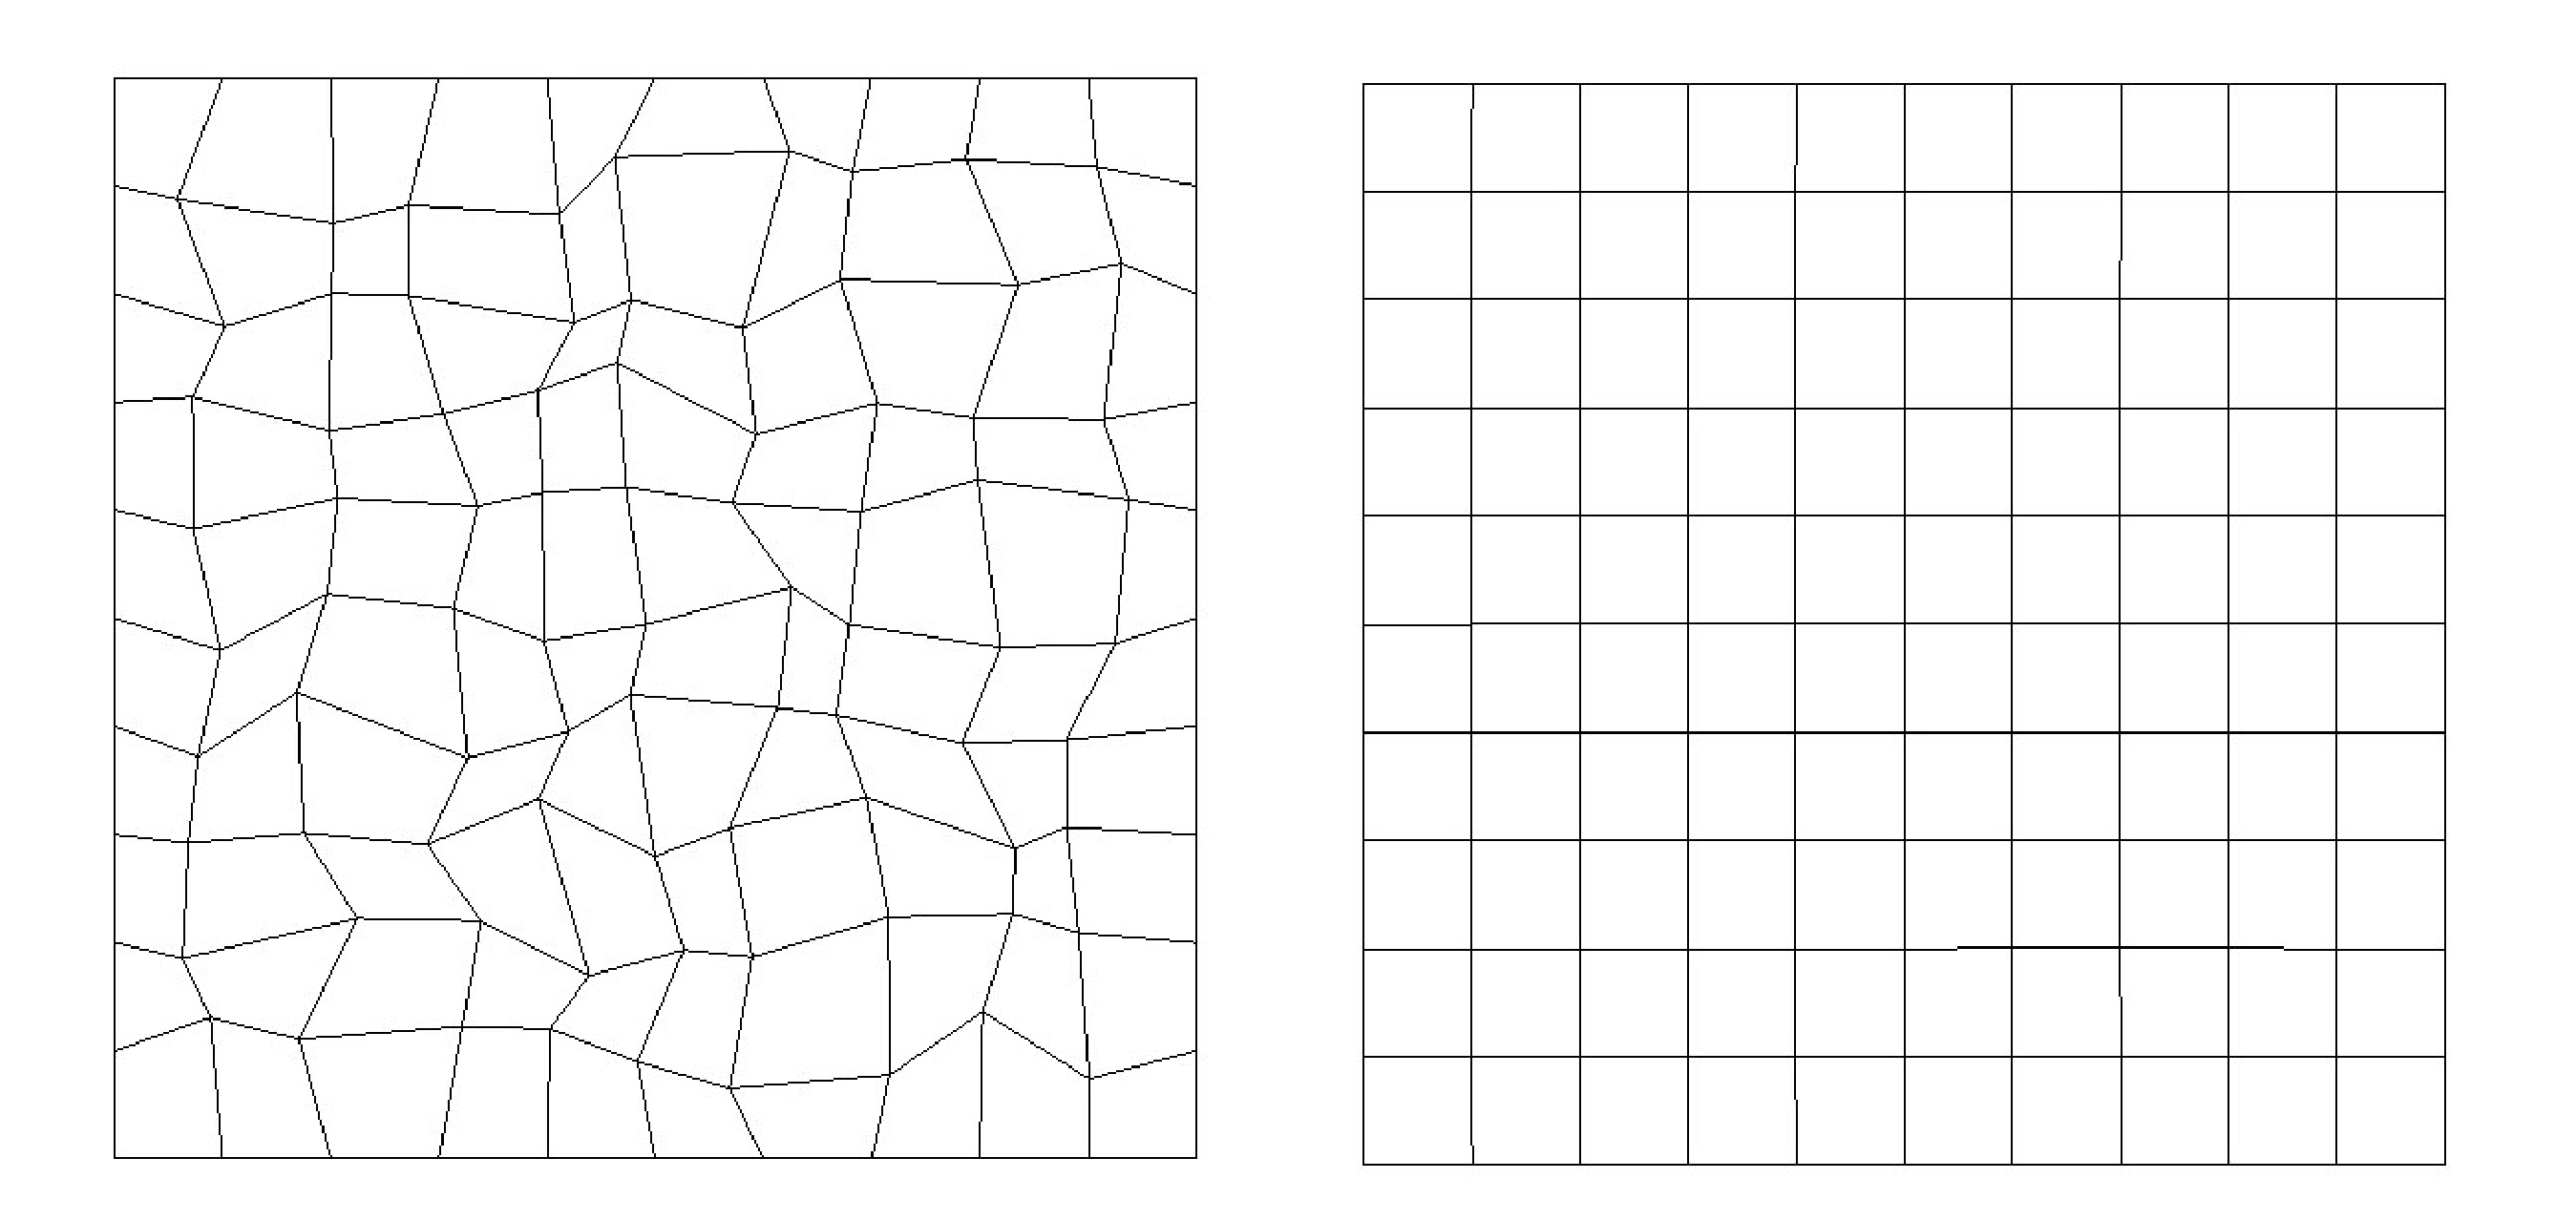
\includegraphics{square_rand.eps}
    \caption{square\_quad\_10\_rand.vtk mesh. The original mesh is on the left, the mesh smoothed with the \texttt{ShapeImprovementWrapper} is shown on the right.}
    \label{fig:square_rand}
\end{center}
\end{figure*}


\subsection{Improving the Mesh with the Low Level API}
\label{sec:tutDetailedAPI}
If the user requires in-depth control over the mesh quality improvement
process, the use of lower-level Mesquite classes provides an extensive
amount of flexibility.   In particular, the user can specify the quality
metric, objective function template, and optimization algorithm by
instantiating particular instances of each.  For each, various options
such as numerical or analytical gradient and Hessian evaluations or
the patch size can be selected.  Furthermore, the user can fine tune
the optimization algorithm performance by creating and setting the parameters 
of the termination criteria.
%for both inner and outer iterations.
%mbrewer removed reference to inner and outer iterations.
%{\tt LAF have we talked about inner and outer iterations before? perhaps
%too advanced for the tutorial}

Once these core objects have been created and customized, the user
creates an instruction queue and adds one or more quality improvers
and quality assessors to it.  The mesh optimization process is initiated
with the {\tt run\_instructions} method on the instruction queue
class.

In this section, we provide a simple example to highlight the main
steps needed for this approach.  The code segment given below performs
the same functionality as the wrapper class highlighted in the
previous section.  The comment lines provide high level documentation;
the details of the each class and the low-level API are extensively
treated in section
\ref{spec:detailedAPI}.

\begin{verbatim}
    // creates a mean ratio quality metric ...
  IdealWeightInverseMeanRatio inverse_mean_ratio(err);MSQ_CHKERR(err);
  inverse_mean_ratio.set_gradient_type(QualityMetric::ANALYTICAL_GRADIENT);
  inverse_mean_ratio.set_hessian_type(QualityMetric::ANALYTICAL_HESSIAN);

    // sets the objective function template
  LPtoPTemplate obj_func(&inverse_mean_ratio, 2, err); MSQ_CHKERR(err);
  obj_func.set_gradient_type(ObjectiveFunction::ANALYTICAL_GRADIENT);
  
    // creates the optimization procedures
  FeasibleNewton f_newton(&obj_func);

    //performs optimization globally
  f_newton.set_patch_type(PatchData::GLOBAL_PATCH, err); 

    // creates a termination criterion and 
    // add it to the optimization procedure
    // outer loop: default behavior: 1 iteration
    // inner loop: stop if gradient norm < eps
  TerminationCriterion tc_inner;
  tc_inner.add_criterion_type_with_double(
    TerminationCriterion::GRADIENT_L2_NORM_ABSOLUTE, 1e-4, err); 
  f_newton.set_inner_termination_criterion(&tc_inner);

    // creates a quality assessor
  QualityAssessor m_ratio_qa(&inverse_mean_ratio,QualityAssessor::AVERAGE,err);
  MSQ_CHKERR(err);
    // creates an instruction queue
  InstructionQueue queue;
  queue.add_quality_assessor(&m_ratio_qa, err); MSQ_CHKERR(err);
  queue.set_master_quality_improver(&f_newton, err); MSQ_CHKERR(err);
  queue.add_quality_assessor(&m_ratio_qa, err); MSQ_CHKERR(err);

    // do optimization of the mesh_set
  queue.run_instructions(mesh_set, err); 
\end{verbatim} 

\subsection{Mesh Improvement Examples}

The left image in figure \ref{fig:hole} shows a mesh that has
been degraded by moving the disk from the right side of the square to
the left while keeping the mesh topology fixed.
The mesh file
\texttt{mesquite/meshFiles/2D/VTK/hole\_in\_square.vtk} contains the
information for this mesh.  If you plan to run this example, note that
the normal direction that defines the geometry is now $(0,0,-1)$.
This change must be made in the tutorial example code
as was done in section \ref{sec:tutMesh}, or an error message will be
thrown.
\begin{verbatim}
  Vector3D normal(0,0,-1);
  Vector3D point(0,0,-5);
  PlanarDomain my_mesh_plane(normal, point, my_mesh);
  mesh_set.set_domain_constraint(&my_mesh_plane);
\end{verbatim}

We can now improve the mesh with the wrapper mentioned in
\ref{sec:tutWrapper} or the detailed API mentioned in
\ref{sec:tutDetailedAPI}. 
Because we changed the normal, the driver code must be recompiled;
otherwise the code and executable are as before.
Once the code is recompiled, type 
\begin{verbatim}
./tutorial ../../meshFiles/2D/VTK/hole_in_square.vtk
\end{verbatim}
to improve this mesh.
The smoothed mesh is shown in the right image of figure
\ref{fig:hole}.
The vertex locations have been repositioned and significantly improve
the quality of the mesh, as shown by the onscreen
quality assessor output:  
\begin{verbatim}
************** QualityAssessor Summary **************

  There were no inverted elements detected. 
  No entities had undefined values for any computed metric.

             metric     average
 Inverse Mean Ratio     85.8391

************** QualityAssessor Summary **************

  There were no inverted elements detected. 
  No entities had undefined values for any computed  metric.

             metric     average
 Inverse Mean Ratio     1.83479

\end{verbatim}
\begin{figure*}[htbp]
\begin{center}
    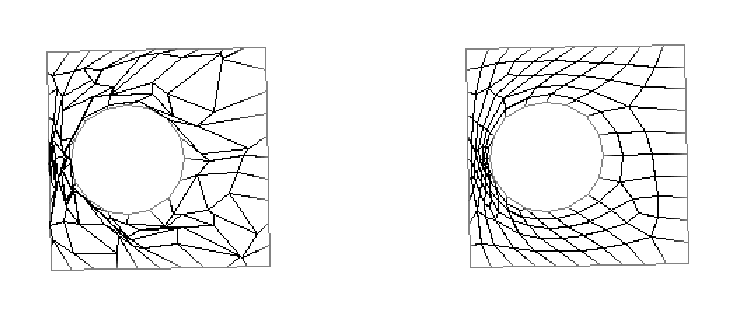
\includegraphics{hole_in_square.ps}
    \caption{hole\_in\_square.vtk mesh. The original mesh is on the left, the mesh smoothed with
    Mesquite is shown on the right.}
    \label{fig:hole}
\end{center}
\end{figure*}
